\chapter{序論}
\label{chap:introduction}

\section{背景}

アプリケーション開発が近年盛んになってる。

デザインの重要性を述べる
%Goodpatchを持ってくる。シリコンバレーは共同創業者にデザイナがいてユーザの体験をきちんと設計していた

そしてデザインは表層のデザインとされがちであるが本質は奥深くにある。
%Goodpatchのダイアグラムを引用

だが

近年,一般市民にとって身近なサービス機能がオンライン化されるにつれ,ソフトウェアのユーザビリティの重要性が認識されるようになっている\cite{kurosu}.総務省の情報通信白書によると2020年までに世界のモバイル向けアプリ市場は売上高で1,924億ドルとなっており,今後も拡大が予測されている.これらの市場はモバイルゲームが牽引してきたが,今後はそれに加えて学習や翻訳,健康管理,SNSなどのアプリケーションも成長が見込まれている\cite{hakusyo}.これらはいずれも消費者向けのサービスであり,業務用サービスに比べ習熟を求めることができず利用者数も多くなる傾向にある.このようなモバイル向けアプリ市場ではデザインや使い勝手が製品の購買の決め手になるためユーザビリティがより重要になる.近年では,機能だけではなく,むしろ使いやすさのコンセプトを全面に押し出して製品を広告したり,製品やブランドの魅力として使いやすさを訴える企業が増えている\cite{tullis2014}.家電メーカーのBalmuda社長の寺尾は次のように述べており,機能性よりも製品から受ける体験を重視した製品を目指している.\begin{quotation}
  現代を生きる私たちは,家電や携帯電話,クルマなど,さまざまな便利な道具に囲まれて暮らしています.しかし,便利であればそれで良いのでしょうか? 人生に本当に必要なのは,驚きや感動,うれしくなるような体験なのだと思います\cite{terao}.
\end{quotation}


また,個人のアプリ利用者の年齢層が年々広がっており,幅広い年齢層にとって使いやすいサービス設計が必要になってきている.インターネットの利用率を年代別に見ると平成19年末時点で6-12歳が68.7\%,50-59歳が81.2\%,60-64歳が63.0\%,65-69歳が36.9\%だったのに対し,令和2年では6-12歳が80.7\%,50-59歳が94.7\%,60-69歳が82.7\%と利用者数の伸びが顕著である\cite{doukou1}\cite{doukou2} .利用者の年齢層が広がることで嗜好や身体の状態,前提知識に大きな幅が生まれることが考えられる.サービス開発者には様々な利用者を想定して設計することが求められ,ユーザビリティの高いデザインの開発がより困難になる.

ユーザビリティについては古くから検討されており,Shackel\cite{shackel1991human}はユーティリティを高めることと同程度にユーザビリティを高めることが重要であると主張している.ユーティリティは機能性(functionality)とも言い換えられ,「機能があっても使いにくいコンピュータ」に対して「使いこなせるか」ということを示すためにユーザビリティの概念を提唱した\cite{kurosu}.その後,ユーザビリティは体系化され,ISO/IEC 25000(別名 SQuaRE)の規格の中に取り込まれ,ソフトウェアの品質基準のひとつとなっている.

Nielsenのユーザビリティエンジニアリング原論ではユーザビリティに配慮した開発では次の工程が例として挙げられている\cite{nielsen2002}.
\begin{enumerate}
  \item ユーザー調査
  \item 競合製品との比較分析
  \item パラレルデザイン
  \item ユーザー参加型デザイン
  \item トータルインタフェースのコーディネートデザイン
  \item ガイドライン・ヒューリスティック評価
  \item プロトタイピング
  \item インタフェース評価
  \item 反復デザイン
  \item インストールしたシステムのフォローアップ調査
\end{enumerate}
この工程では,実際の開発であるプロトタイピングの前にヒューリスティック評価,その後インタフェース評価とフォローアップ調査と3つのポイントでユーザビリティ評価を行っている.このように,ユーザビリティの高いシステムを開発するには,ヒューリスティクス(経験則)に基づいてユーザビリティを検討しデザインするのに加え,実際に開発したシステムのインタフェースのユーザビリティを評価し,修正する反復的な作業が必要になる.さらに,システムの導入後も調査を行い,さらに反復的に改善していくことが重要である.

ユーザビリティの評価では,ユーザに直接使用させて評価することは欠かすことができない重要な工程である.Nielsenのヒューリスティック評価\cite{nielsen1990}では,多くのユーザが共通して使いやすいと感じるであろう項目を挙げ,それらを満たしたシステムを開発することでユーザビリティの向上を目指している.しかし,この手法では適用できる範囲に限界があるだけでなく,そもそもユーザの多様性を考慮して設計することができない.ここでの多様性とは,障害者や高齢者というだけでなく,年齢や性別などの特性,嗜好や価値観などの指向性,精神状態や物理的環境などユーザのあらゆる違いを含んでいる\cite{kurosu2013}.これらのユーザそれぞれがシステムの利用に際して起こることについてはヒューリスティクスでは網羅できていない.そこで,製品のターゲットとなるユーザを被験者として集め,実際にシステムを操作してもらうユーザテストが行われる.

ユーザテストでは,ユーザビリティに関連する様々な指標を測定することでユーザビリティを評価する.測定手法はパフォーマンスメトリクス,自己申告メトリクス,行動・生理メトリクスに分類することができる\cite{tullis2014}.パフォーマンスメトリクスとは,タスク成功率,タスク時間,エラー頻度,効率,学習可能性などで,定量的に計測できるため測定が容易である.自己申告メトリクスはリッカート尺度による質問紙や自由記述などのアンケートであり一般的に行われている.行動・生理メトリクスは,言語行動と非言語行動を観察したりセンサー等を用いて観測するものである.具体的にはビデオの録画や筋電位センサー,アイトラッキング,皮膚伝導率,心拍数などが指標として使われている\cite{tullis2014}.これらの測定手法は,複数の手法を組み合わせて補完的に活用していく必要がある.

近年,UXが話題になっていることに代表されるように,ユーザの主観的側面が注目されており,ユーザテストへの導入も検討されている.前述の測定手法では,自己申告メトリクスと行動・生理メトリクスが主観的側面に注目した手法といえる.Jordanは前述の機能性とユーザビリティに加えて``嬉しさ''の重要性を述べており,ユーザは機能がありユーザビリティが満たされると嬉しさを要求すると述べている\cite{jordan2000designing}.黒須はISO/IEC 25010:2011の品質特性の図を改良し図\ref{fig:kurosu2015}のような品質特性図を提案している\cite{kurosu2015}.この中では,設計品質をUI,利用品質をUXと便宜上分けており,さらに利用品質の中に定量的に測定可能な客観的利用品質と直接測定できない主観的利用品質を置いている.利用品質のうち,客観的利用品質についてはパフォーマンスメトリクスといった手法で測定が可能になっており,主観的利用品質については自己申告メトリクスや行動・生理メトリクスが活用できる.自己申告メトリクスだけではユーザが全てを申告できなかったりバイアスがかかりやすいことから十分とはいえず,行動・生理メトリクスなど他の測定手法を併用する必要がある.しかし,ユーザの主観を正確に測定する方法は様々なものが提案されているものの一般に普及しているとはいえない.

\begin{figure}[htbp]
  \begin{minipage}{\hsize}
    \begin{center}
       \fbox{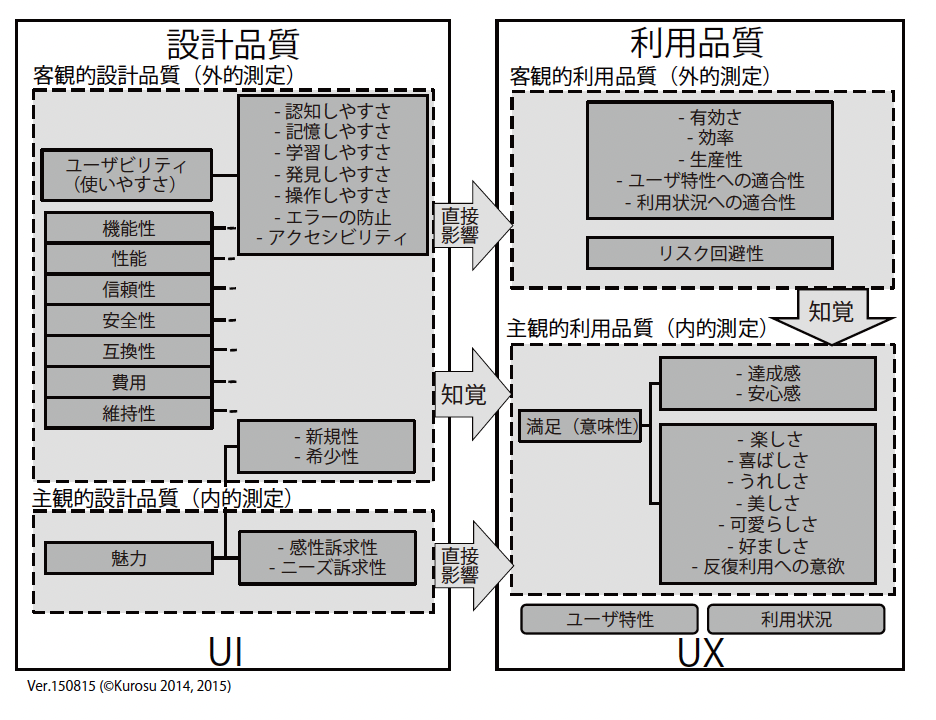
\includegraphics[width=100mm]{img/kurosu2015.png}}
    \end{center}
    \caption{黒須の品質特性図 画像入れ直すこと}
    \label{fig:kurosu2015}
  \end{minipage}
\end{figure}

このように,ユーザビリティ及びUXの評価はユーザにとって使いやすいシステムの開発に不可欠なものであり,その評価手法は定着しているもの,定着していないものを含めて様々に存在しているが,実際の開発ではUXの評価は大規模な消費者向けサービスを除いてほとんど行われていないか,行われていても改善に役立てられていないのが現状である.黒須\cite{kurosu}は,\begin{quotation}
  著者が企業における実態を調べると,そもそもUX調査を実施していることが稀というほど少なく,さらに実施していても,それを担当した部署と企画や分析を担当する部署との間の連携が取れておらず,せっかく取得した実利用に関する情報が企画やユーザ理解にもとづく具体化に役に立っていないことがわかった.
\end{quotation}と述べている.また,UX品質保証サービスを提供する企業が2020年にソフトウェア開発企業の社員490名を対象に行った調査では,UX向上に取り組んでいると応えた割合は34\%に留まっており,UXの評価を行っている割合は更に少ないと考えられる.実ユーザの体験を調査せずにユーザの満足性が高いシステムを開発することはできないため,小規模の開発でもUX評価を行えるようにする必要がある.

また,UXはユーザ毎に異なるだけでなく,使用の前,使用中,習熟後などのステージや折々の出来事によって変化するため,変化を考慮して評価する必要がある\cite{kurosu}.黒須はこのようなUXの変化を記述,視覚化するためにUXグラフ\cite{kurosu2015}を提案している.このUXグラフはユーザが製品を数週間から数ヶ月といった長期間にわたって使用した体験を,縦に満足性,横を時間軸にしてカーブで表すものである.一方で,システムを使用している数分間から1時間程度の期間の変化についてはユーザに変化を記述させることが難しくUXグラフは使われていない.しかし,UXの概念では,時間軸の変化は重要な要素であり,短期間の使用時であってもそれを評価する方法が必要であると考えられる.

以上のことから,(1)現在は大規模な開発でしか行われていないユーザテストの導入ハードルを下げ普及させること,(2)UXの重要な部分である満足性を測定する簡便な手法を開発すること,(3)(2)で測定した満足性からUXの時間変化を記録し可視化する手法を開発することが求められる.

\section{目的}

本研究では(1)現在は大規模な開発でしか行われていないユーザテストの導入ハードルを下げ普及させるために,UX評価や統計処理についての専門的な知識が無くても容易にユーザテストを行いシステムの問題点を発見できるようにするシステムの開発を目指す.行動・生理メトリクスは確立された手法が無いため普及していないものの,分析の自動化と相性が良いため手法さえ確立できれば容易なユーザテスト手法になり得る.ユーザビリティテストでは,被験者は笑ったりそわそわしたり調査票に記入するよりもはるかに多くの行動を行うがそれらを記録することでより情報量の大きいデータを入手可能になる\cite{tullis2014}.そこで,(2)及び(3)の手法を用いて統合的な分析システムを開発する.

(2)満足性を測定する新たな簡便な手法として,容積脈波でストレスを測定する手法の満足性評価への応用を提案する.行動・生理メトリクスは満足性と関係があると考えられ,これまでにも皮膚伝導率や心拍数を用いてストレスで満足性を評価する手法が提案されてきた.容積脈波は,カオス解析することで鬱やパーキンソン病の診断に活用できる可能性が指摘されている\cite{tuan}\cite{oyama}.さらに,同様の解析により精神状態を測定できる可能性\cite{arai}が指摘されていることから,従来の皮膚伝導率や心拍数などのシンプルな方法よりも高精度なストレス測定が期待できる.また,脳波を用いてストレスを測定しユーザビリティを評価する手法\cite{amaral}も提案されているが,装置が大がかりになるために導入にコストがかかったり,測定器を装着すること自体がストレスになる可能性がある.そのため,耳朶に装着する小型のセンサーで容積脈波を取得しストレスを測定,満足性を評価する方法を提案する.これに基づき,容積脈波を解析して得たストレス指標と従来のユーザビリティ指標の関係を示した.

短期間のUX変化を黒須のUXグラフで表記させることは難しいが,容積脈波から得られるストレス指標のような生理メトリクスであればシーケンシャルであるため(3)使用中のUXの時間変化を記録し可視化することが可能になる.容積脈波を解析しストレスを算出するシステムであるLyspect\cite{oyama2012}では,ストレス指標の時系列変化を出力することができなかった.そこで容積脈波をリアルタイムで取得し,解析して得られるストレス変化を時系列グラフで表示するシステムを開発した.そして,開発したシステムの有効性を示した.

\section{本論文の構成}

本論文の構成を示す.

第\ref{chap:introduction}章では本研究の背景について述べた.第\ref{chap:prevresearch}章では関連研究と諸概念を整理する.第\ref{chap:pulsewave}章では脈波によるストレスチェックを応用したユーザビリティ評価手法を提案し,第\ref{chap:pulsewave}章ではそれを発展させた時系列ユーザビリティ評価手法を提案する.そして,それらの有効性を示す.最後に,第\ref{chap:conclusion}章の結論では本研究を総括し,考察と展望を述べる.付録として,本研究で行った実験で得られたデータを添付する.
